\chapter{淋巴造血系统疾病}

\chapterabstract{本章主要介绍淋巴造血系统的两类恶性肿瘤:恶性淋巴瘤和白血病。要求掌握恶性淋巴瘤的概念及分类、霍奇金淋巴瘤的病变特点和组织学类型,白血病的概念及主要类型;熟悉非霍奇金淋巴瘤的分类及其病理改变、急性白血病的分类、病理改变及临床表现;了解慢性白血病的分类、病理改变及临床表现。}

淋巴造血系统包括髓性组织(myeloid)和淋巴组织(lymphoid
tissue)两个部分,髓性组织主要由骨髓和血液中的各种血细胞成分构成,包括红细胞和白细胞(粒细胞、淋巴细胞、单核细胞等)。淋巴组织包括胸腺、脾脏和淋巴结及在人体广泛分布的淋巴组织,如扁桃体、腺样体、肠黏膜固有层的集合和孤立淋巴小结群等。

本章主要介绍源于这两种淋巴造血组织的恶性肿瘤性疾病。

\begin{framed}
{案例9-1}

{【病例摘要】}

患者,女,26岁,因左侧颈部肿块渐增大半年入院。期间曾给予抗感染治疗,无明显效果。既往无特殊病史。体检:可见双颈部多发性肿大淋巴结,左颈部淋巴结巨大,质硬,已广泛融合固定,大小约12
cm×6
cm,延伸至颈后,双侧锁骨上均触及肿大淋巴结,质软,无压痛,表面光滑,活动可,大小约1.2
cm×1
cm。颈部CT(增强)示:两侧颈部、两侧锁骨上及左侧腋下多发淋巴结肿大。

{【问题】}

(1)若欲确诊,尚需哪些检查?

(2)该患者可能的病理诊断及镜下病理形态是什么?
\end{framed}

\section{淋巴瘤}

\subsection{概述}

淋巴瘤(lymphoma)也称恶性淋巴瘤(malignant
lymphoma,ML),是指原发于淋巴结和结外淋巴组织等处的淋巴细胞及其前体细胞克隆性增生而形成的一类恶性肿瘤。根据瘤细胞的形态、免疫表型和分子生物学特点,可将其分为霍奇金淋巴瘤(Hodgkin
Lymphoma,HL)和非霍奇金淋巴瘤(non-Hodgkin
Lymphoma,NHL)两大类。后者包括前体B和T细胞肿瘤、成熟B细胞肿瘤、成熟T和NK细胞肿瘤等,绝大多数为B细胞源性,其次为T/NK细胞源性,而组织细胞性肿瘤罕见。

淋巴瘤在我国占所有恶性肿瘤的3%~4%。近年来淋巴组织肿瘤的发病在国内外均呈上升趋势。

\subsection{WHO关于淋巴瘤的分类}

WHO关于淋巴瘤分类(2008)以细胞系为线索,是集淋巴细胞、髓细胞、组织细胞与树突状细胞和肥大细胞的肿瘤于一体的分类。该分类将肿瘤的组织病理学、免疫学表型、遗传学特征和临床表现相结合来确定每一个独立亚型;根据淋巴瘤的病变范围及其生物学行为,引进了惰性(indolent)、侵袭性(aggressive)和高侵袭性(highly
aggressive)淋巴瘤的概念,更容易为临床医生所理解。

在WHO分类中,根据肿瘤细胞的起源,淋巴组织肿瘤被分为前体B细胞肿瘤(不成熟B细胞肿瘤)、外周B细胞肿瘤(成熟B细胞肿瘤)、前体T细胞肿瘤(不成熟T细胞肿瘤)、外周T细胞肿瘤(成熟T细胞肿瘤)和霍奇金淋巴瘤,详见表\ref{tab9-1}\footnote{此为简化版。引自Robbin's Basic Pathology(9th ed)。}。

\begin{table}[ht]
    \caption{WHO关于淋巴组织肿瘤的分类(2008)}
    \label{tab9-1}
    \centering
    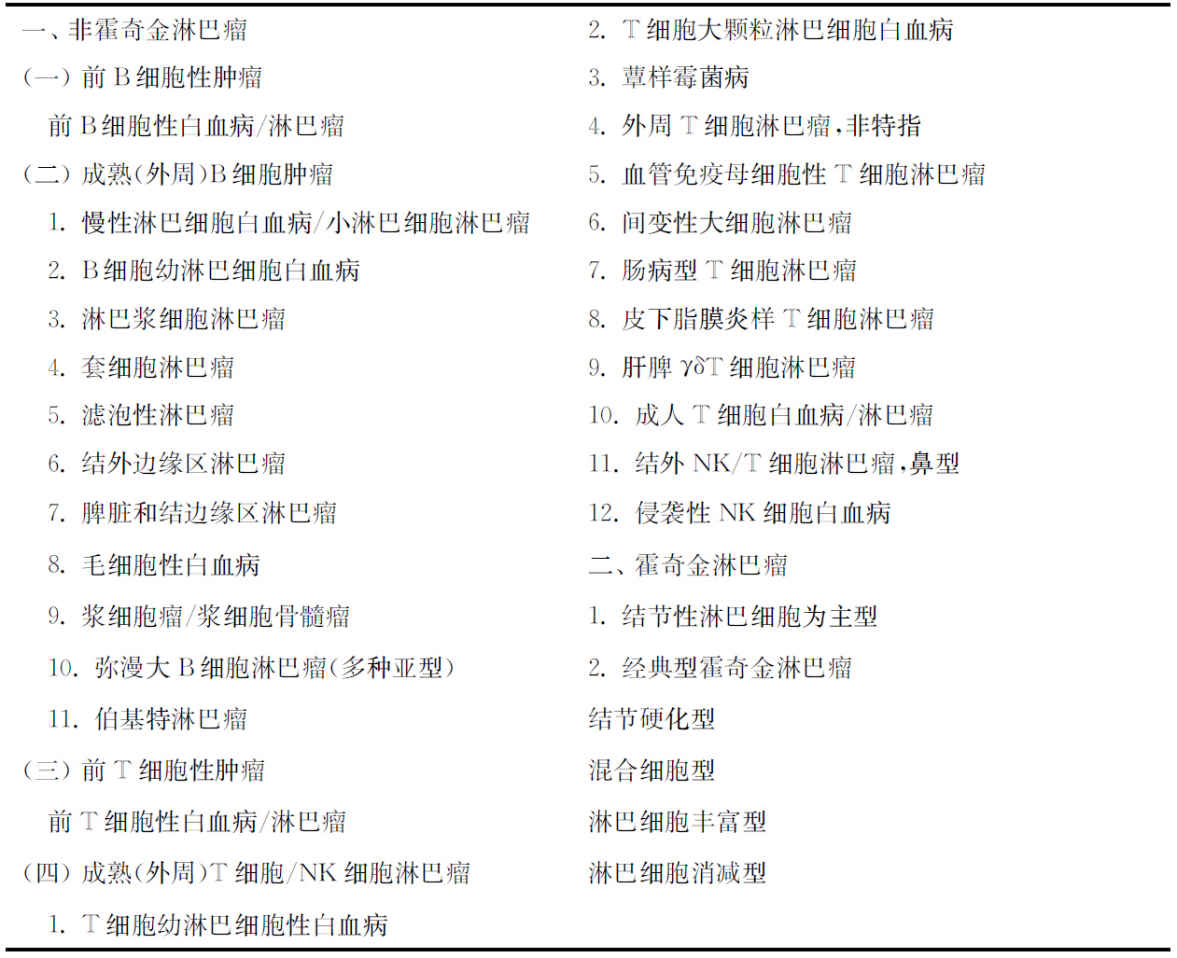
\includegraphics{./images/Image00140.jpg}
\end{table}

\subsection{淋巴瘤的临床分期}

关于淋巴瘤的临床分期,目前仍使用的是1971年在Ann
Arbor召开的关于HL的临床治疗工作会议上制定的、Costwolds(1989)修改的临床分期,Ann
Arbor分期系统也同样适用于NHL,详见表\ref{tab9-2}。

\begin{longtable}[ht]{cp{7cm}}
    \caption{淋巴瘤的临床分期(Ann Arbor,1971)}
    \label{tab9-2}\\
    \toprule
    分期 & 肿瘤累及范围\\
    \midrule
    I期&病变局限于以组淋巴结(I)或一个结外器官或部位(I$_E$)\footnote{E:结外(exranodal)}\\
II期&病变局限于膈肌同侧的两组或两组以上的淋巴结(II)或直接蔓延至一个结外器官或部位(II$_E$)\\
III期&累及膈肌两侧的淋巴结(III)或再累及一个结外器官或部位(III$_E$)或脾脏(III$_S$)或两者(III$_{SE}$)\\
IV期&弥漫或播散性累及一个或多个结外器官.如骨髓和胃肠道等\\
    \bottomrule
\end{longtable}
      


\subsection{非霍奇金淋巴瘤}

非霍奇金淋巴瘤(NHL)占所有淋巴瘤的80%~90%,其中2/3原发于淋巴结,1/3原发于淋巴结外器官或组织,如消化道和呼吸道、肺、皮肤、涎腺、甲状腺和中枢神经系统等(图\ref{fig9-1})。与HL不同之处在于发病部位的随机性或不定性,肿瘤扩散的不连续性,组织学分类的复杂性和临床表现的多样性。在某些NHL,淋巴瘤与淋巴细胞白血病有重叠,两者为同一疾病的不同发展阶段。

\begin{figure}[!htbp]
 \centering
 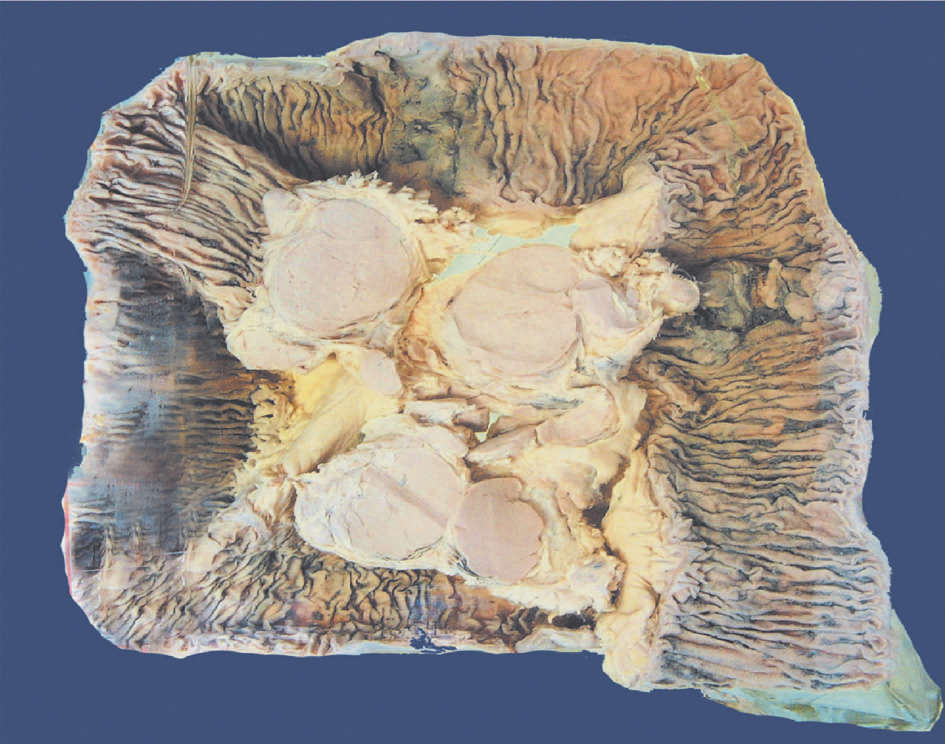
\includegraphics{./images/Image00142.jpg}
 \captionsetup{justification=centering}
 \caption{肠系膜淋巴结非霍奇金淋巴瘤\\ {\small 肿瘤切面细腻,鱼肉样}}
\label{fig9-1}
  \end{figure}

在我国发生在成人淋巴结的NHL主要是弥漫大B细胞淋巴瘤;在儿童和青少年则是急性淋巴母细胞白血病/淋巴瘤和Burkitt淋巴瘤;淋巴结外淋巴瘤主要有黏膜相关淋巴瘤和鼻型NK/T细胞淋巴瘤,前者主要发生在胃肠道、涎腺和肺等,后者主要累及中线面部的器官和组织。下面将对当前我国常见的一些NHL类型进行介绍。

\subsubsection{外周(成熟)B细胞肿瘤}

\paragraph{弥漫大B细胞淋巴瘤}
弥漫大B细胞淋巴瘤(diffuse large B-cell
lymphoma,DLBCL)是一组异质性B细胞淋巴瘤,是最常见的NHL,占所有NHL的30%~40%。

(1)病理改变:相对单一形态、体积较大的瘤细胞弥漫浸润,其直径为小淋巴细胞的4~5倍。细胞形态多样,类似中心母细胞、免疫母细胞、间变大细胞或浆母细胞(图\ref{fig9-2})。核圆形或卵圆形,染色质边集,有单个或多个核仁。胞浆中等,嗜碱性。也可有间变性的多核瘤细胞出现,类似霍奇金淋巴瘤或R-S细胞。肿瘤细胞表达B细胞分化抗原CD19、CD20和CD79a,多数表达表面免疫球蛋白(SIg),不表达末端脱氧核苷酸转移酶(terminal
deoxynucleotidyl transferase,TdT)。

\begin{figure}[!htbp]
 \centering
 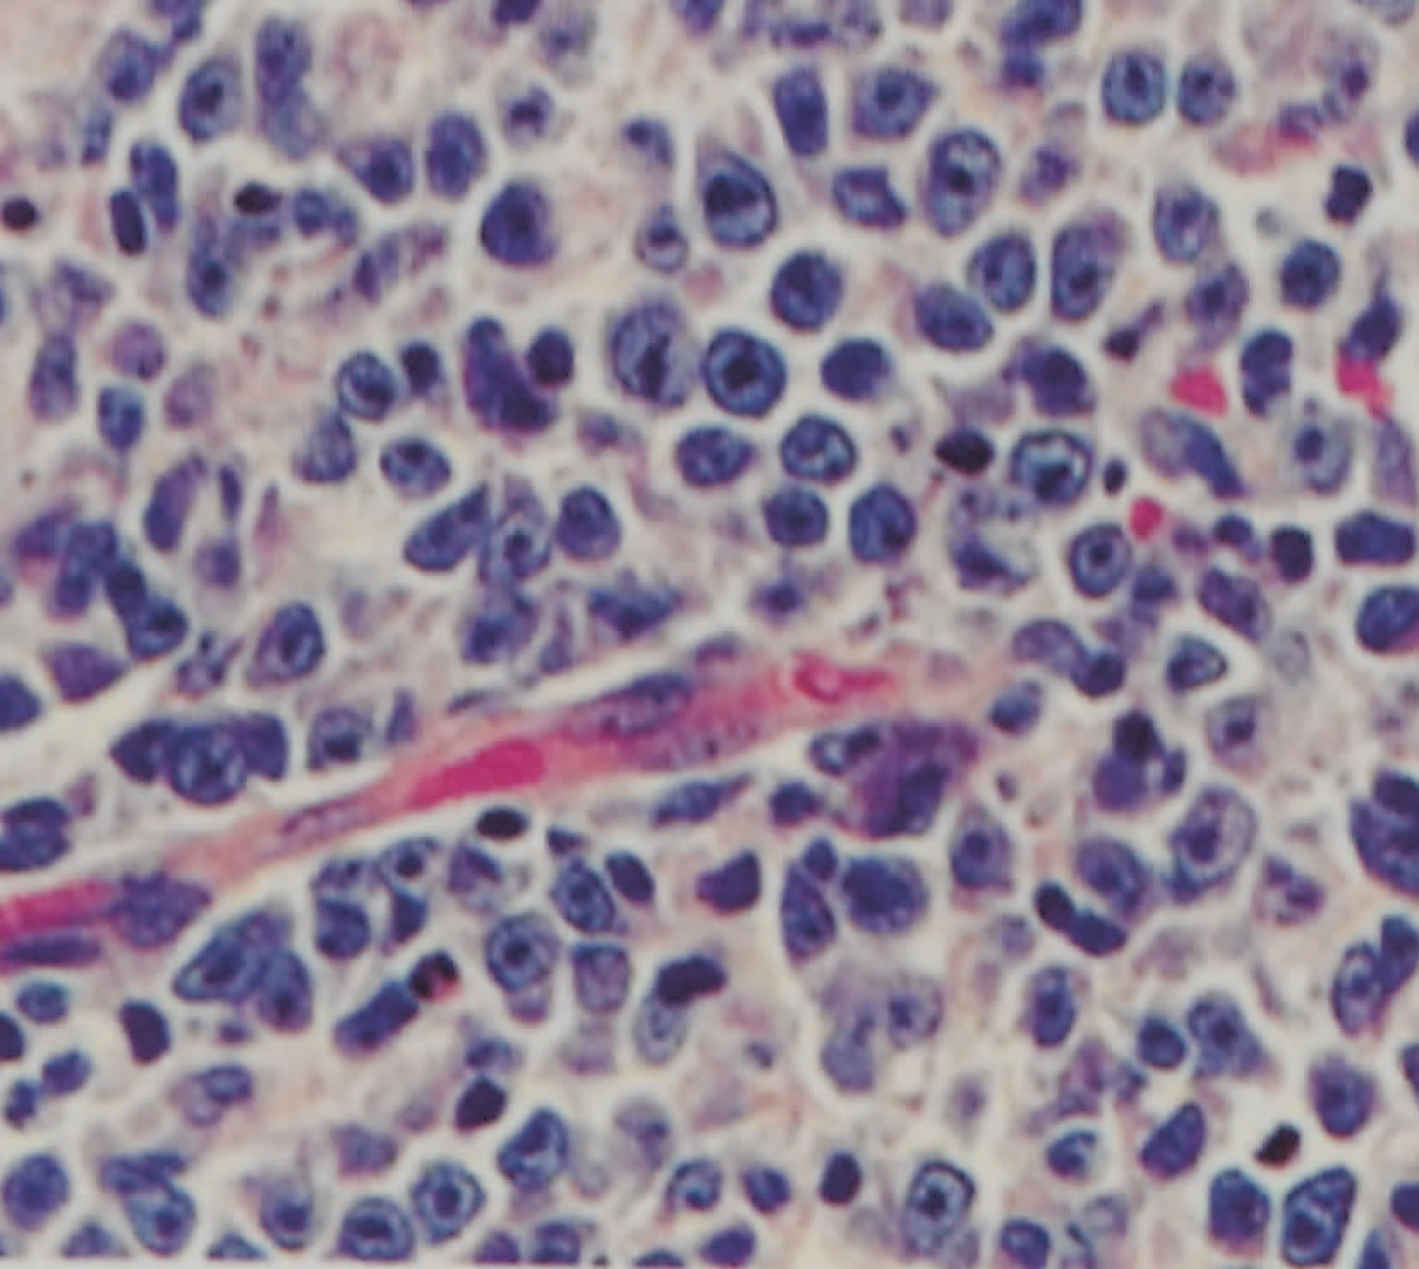
\includegraphics{./images/Image00143.jpg}
 \captionsetup{justification=centering}
 \caption{弥漫大B细胞淋巴瘤(HE染色,高倍)\\ {\small 摘自《WHO造血与淋巴组织肿瘤分类》(第4版)肿瘤细胞形态学表现一致,中位核仁}}
\label{fig9-2}
  \end{figure}

(2)临床表现:老年男性患者略多,平均年龄60岁。常在短时期内出现淋巴结迅速长大或结外肿块。病情进展迅速,可累及肝脾,但骨髓受累者少见。该肿瘤除原发于淋巴结外,还可原发于纵隔、口咽环、胃肠道、皮肤、骨和脑等处。DLBCL是一种侵袭性肿瘤,若未及时诊断和治疗,患者会在短期内死亡。一般采用强化治疗,60%~80%的患者可完全缓解,约50%的患者可达临床痊愈。

\paragraph{滤泡性淋巴瘤}
滤泡性淋巴瘤(follicular
lymphoma,FL)是滤泡生发中心细胞来源的惰性B细胞肿瘤,欧美国家常见,占所有NHL的25%~45%。在中国,约占NHL的10%~13%。

(1)病理改变:FL的组织学特征是在低倍镜下肿瘤细胞常呈明显的结节状生长方式。肿瘤性滤泡主要由中心细胞和中心母细胞以不同比例组成。中心细胞的细胞核形态不规则、有裂沟,核仁不明显,胞质稀少;中心母细胞的体积比正常淋巴细胞大3~4倍,核圆形或分叶状,染色质呈斑块状近核膜分布,有1~3个近核膜的核仁。多数FL的肿瘤细胞是中心细胞,随着病程的进展,中心母细胞数量逐渐增多。生长方式从滤泡型发展成弥漫型,提示肿瘤侵袭性增高。FL的肿瘤细胞表达CD19、CD20、CD10和单克隆性的SIg。约90%的病例之肿瘤细胞表达Bcl-2蛋白,而正常滤泡生发中心B细胞为Bcl-2阴性。几乎所有肿瘤细胞都表达Bcl-6。因此,Bcl-2蛋白也是区别反应性增生的滤泡和FL的肿瘤性滤泡的有用标记。

(2)临床表现:FL常见于中年人。主要表现为局部或全身淋巴结无痛性肿大,以腹股沟淋巴结受累多见。常有脾脏大,部分患者发热和乏力等。30%~50%的病例有骨髓受累,但不影响预后。尽管FL难以治愈,强化治疗也不会改善病情,但在临床上表现为惰性过程,病情进展缓慢,预后较好。5年生存率超过70%。30%~50%的患者可转化为DLBCL。

\paragraph{Burkitt淋巴瘤}
Burkitt淋巴瘤(Burkitt
lymphoma,BL)是淋巴滤泡生发中心细胞来源的高侵袭性B细胞肿瘤。其发病与EB病毒感染密切相关。

(1)病理改变:BL的组织学特点是淋巴结结构破坏,中等大小、相对单一形态的淋巴细胞弥漫性浸润。瘤细胞核圆或卵圆形,直径相当于反应性组织细胞的核,有三到五个明显的核仁,染色质比较粗糙。胞质中等量,HE染色呈双色性。瘤细胞间散在分布着吞噬有核碎片的巨噬细胞,构成所谓满天星图像。瘤细胞表达成熟B细胞分化抗原,如CD19、CD20、CD79a,表达滤泡生发中心细胞标记Bcl-6和CD10等。表达IgM;表达单一Ig轻链蛋白。用反映细胞增殖活性的Ki-67抗体染色,瘤细胞几乎100%阳性。所有的BL都存在与第8号染色体上c-myc基因有关的异位。

几乎所有的地方性BL都存在EB病毒隐性感染,约25%的HIV相关肿瘤和15%~20%的散发性BL也伴有EB病毒感染。

(2)临床表现:BL多见于儿童和青少年,肿瘤常发生于淋巴结外的器官和组织,可表现为颌面部巨大包块,以及腹腔脏器的受累等。BL属高侵袭性肿瘤,但对短期、大剂量化疗反应好,多数儿童和年轻患者可治愈,但在年长者多预后不良。

\subsubsection{外周T和NK细胞肿瘤}

\paragraph{非特指外周T细胞淋巴瘤}
非特指外周T细胞淋巴瘤(peripheral T-cell
lymphoma,un-specified,PTCL-U)是胸腺后成熟T淋巴细胞来源的肿瘤。在WHO分类中,除已单列的、有独特的临床病理表现的T细胞淋巴瘤以外的所有外周T细胞淋巴瘤均归于此项下。因此,PTCL-U是一组异质性的侵袭性肿瘤。

病理改变:淋巴结结构破坏,瘤细胞在副皮质层或弥漫浸润,有较多的高内皮血管,瘤细胞侵入血管现象。背景中可见嗜酸性粒细胞、浆细胞、组织细胞和上皮细胞等,胶原纤维穿插分隔病变组织。瘤细胞的大小和形态各异,细胞核形态极不规则,可见核扭曲或多分叶状,核染色质呈粗颗粒状,部分瘤细胞有明显的核仁,核分裂象多见。

瘤细胞表达T细胞分化抗原,如CD2、CD3、CD45RO和CD43等。大多数病例有TCR基因的克隆性重排。常可见染色体数量和结构的异常。

\paragraph{NK/T细胞淋巴瘤}
NK/T细胞淋巴瘤(natural killer/T-cell
lymphoma)被认为是自然杀伤细胞来源的侵袭性肿瘤,约2/3的病例发生于中线面部,发生在其他部位者称为结外鼻型NK/T细胞淋巴瘤。在中国,该肿瘤约占所有NHL的15%,属EB病毒相关淋巴瘤。

病理改变:该肿瘤的基本病理改变是在凝固性坏死和混合炎细胞浸润的背景上,肿瘤性淋巴细胞散布或呈弥漫性分布。瘤细胞大小不等、形态多样、细胞核形态不规则,核深染,不见核仁或呈圆形,染色质边集,有1~2个小核仁。瘤细胞可浸润血管壁而致血管腔狭窄或闭塞。肿瘤细胞表达部分T细胞分化抗原如CD2、CD45RO、CD3;表达NK细胞相关抗原CD56,以及细胞毒性颗粒相关抗原,如T细胞内抗原1(T-cell
intracellular antigen1,TIA-1)、穿孔素(perforin)和粒酶B(granzyme
B)等。

\subsection{霍奇金淋巴瘤}

霍奇金淋巴瘤(Hodgkin Lymphoma,HL),亦称霍奇金病(Hodgkin's
disease,HD),是一个独特的淋巴瘤类型,占所有淋巴瘤的10%~20%。其特点:①约90%的病例原发于淋巴结,病变往往从一个或一组淋巴结开始,逐渐由近及远地向附近的淋巴结扩散;②HL的肿瘤细胞是一种独特的瘤巨细胞即Reed-Sternberg
cell(R-S
cell)(图\ref{fig9-3}),瘤细胞在病变组织的所有细胞成分中仅占1%~5%;③HL病变组织中常有不等量的各种炎细胞存在和不同程度的纤维化;④在HL的后期,约10%的病例可累及骨髓;⑤目前的研究结果证实HL的肿瘤细胞具有生发中心或生发中心后B淋巴细胞的特征,故HL实为一类B细胞肿瘤。

\begin{figure}[!htbp]
 \centering
 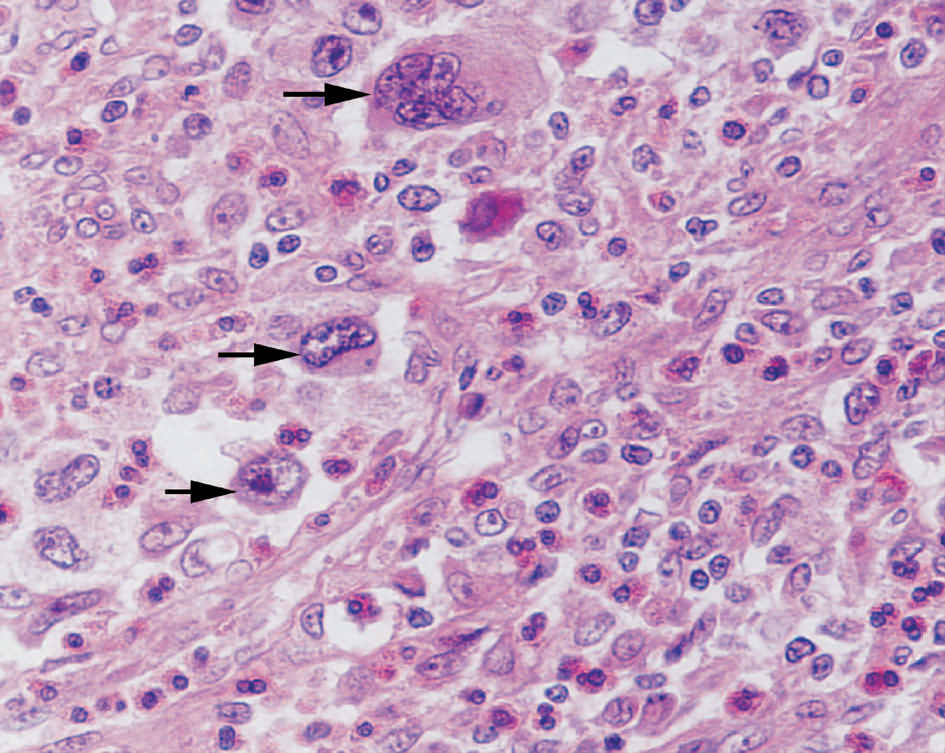
\includegraphics{./images/Image00144.jpg}
 \captionsetup{justification=centering}
 \caption{霍奇金淋巴瘤(HE染色,高倍)\\ {\small 肿瘤组织由R-S细胞(箭示较典型者)和各种反应性炎细胞组成}}
\label{fig9-3}
  \end{figure}

\subsubsection{病理改变}

HL多发生于颈部和锁骨上淋巴结,其次是腋下、纵隔、腹膜后和主动脉旁淋巴结等。首发症状是局部淋巴结的无痛性、进行性肿大。晚期可累及脾、肝和骨髓等器官,以脾脏受累最多见。

\paragraph{大体改变}
受累淋巴结肿大,随着病程进展,相邻的肿大淋巴结彼此粘连、融合,直径可达到10
cm以上,不活动。若发生在颈淋巴结时,可形成包绕颈部的巨大肿块,随着纤维化程度的增加,肿块质地由软变硬。肿块常呈结节状,切面灰白色呈鱼肉样。

\paragraph{镜下改变}
HL的组织学特征是以多种反应性炎细胞混合浸润为背景,数量不等的、形态不一的肿瘤细胞散布其间。肿瘤细胞包括R-S细胞及其变异型细胞。典型的R-S细胞(诊断性R-S细胞)是一种直径15~45
μm的双核或多核瘤巨细胞。瘤细胞胞质丰富,略嗜酸或嗜碱性,核圆形或椭圆形,双核或多核。染色质沿核膜聚集呈块状,核膜厚。核内有一大而醒目的、直径与红细胞相当的、包涵体样的嗜酸性核仁,核仁周围有空晕。典型的双核R-S细胞其双核呈面对面排列,彼此对称,形成所谓“镜影细胞”(mirror
image
cell)(图\ref{fig9-4})。除了典型的R-S细胞外,具有上述形态特征的单核瘤巨细胞称为霍奇金细胞(Hodgkin
cell),这类细胞的出现提示HL的可能。其他变异型的R-S细胞常见于HL的某些亚型中:①陷窝细胞(lacunar
cells),瘤细胞体积大,胞质宽而空亮,核多叶有皱褶,核膜薄,染色质稀疏,有一个或多个较小的嗜碱性核仁。胞质空亮是由于甲醛固定后胞质收缩至核膜附近所致;②L\&H型细胞(lymphohistiocytic
variant,L\&H),亦称“爆米花”细胞(popcorn
cells),瘤细胞的体积大,多分叶状核,染色质稀少,有多个小的嗜碱性核仁,胞质透明;③多核瘤巨细胞,瘤细胞体积巨大,形态不规则,染色质粗,常可见大而明显的、嗜酸性的包涵体样核仁。常见多极核分裂。R-S细胞的死亡方式是凋亡,凋亡细胞皱缩,核固缩,即所谓木乃伊化,又称干尸细胞。

\begin{figure}[!htbp]
 \centering
 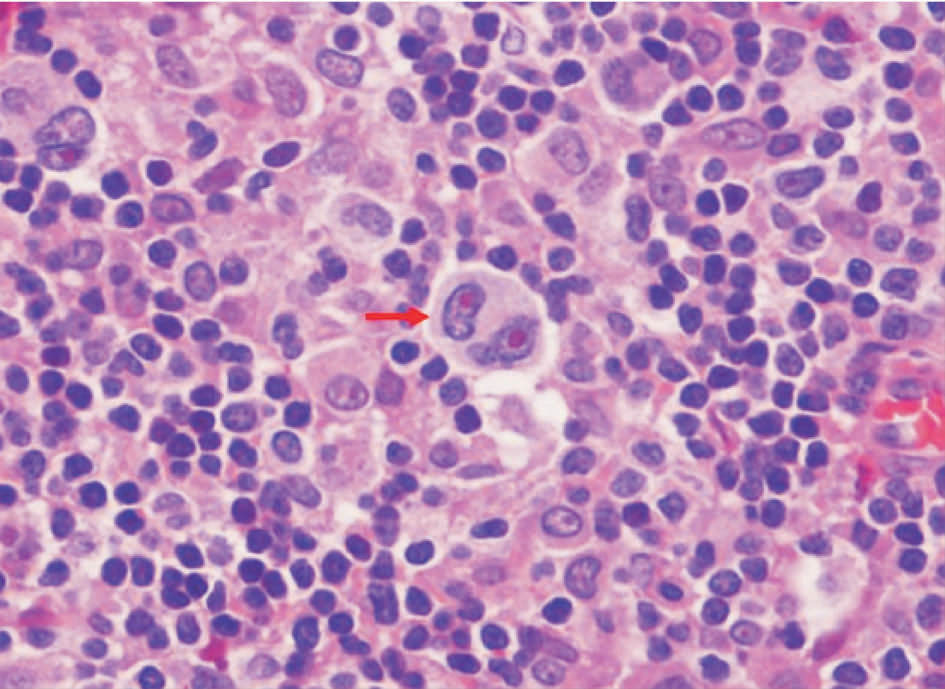
\includegraphics{./images/Image00145.jpg}
 \captionsetup{justification=centering}
 \caption{霍奇金淋巴瘤(HE染色,高倍)\\ {\small 肿瘤组织由R-S细胞和大量淋巴细胞组成,箭头示镜影细胞}}
\label{fig9-4}
  \end{figure}

\subsubsection{组织学分型}

在WHO分类中,将HL分为经典型霍奇金淋巴瘤(classical Hodgkin
Lymphoma,CHL)和结节性淋巴细胞为主型霍奇金淋巴瘤(nodular lymphocyte
predominance Hodgkin
Lymphoma,NLPHL)两大类,根据病变组织中肿瘤细胞核淋巴细胞的数量和比例,以及组织构象特征等,又将CHL分为四个组织学亚型,即结节硬化型、混合细胞型、富于淋巴细胞型和淋巴细胞消减型;经典型霍奇金淋巴瘤的瘤细胞表达CD30(80%)和CD15(70%),而不表达B细胞分化抗原,如CD20、CD79a;结节性淋巴细胞为主型霍奇金淋巴瘤之瘤细胞特征性地表达B细胞的免疫表型,而不表达CD15,少有表达CD30。

\paragraph{结节性淋巴细胞为主型霍奇金淋巴瘤(NLPHL)}
约占所有HL的5%。病变淋巴结呈深染的模糊不清的结节状,典型R-S细胞难觅,常见的是多分叶核的爆米花细胞,即L\&H型细胞。嗜酸性粒细胞、中性粒细胞和浆细胞少见,几乎无坏死和纤维化。瘤细胞表达B细胞标记,不表达CD15,偶表达CD30。3%~5%的病例可转化为弥漫大B细胞瘤。不伴EB病毒感染。NLPHL患者多为男性,年龄小于35岁。主要表现是颈和腋下肿块,预后极好,10年生存率高达80%。

\paragraph{经典型霍奇金淋巴瘤}
(1)结节硬化型(nodular
sclerosis,NS):多见于年轻女性,好发于颈部、锁骨上,特别是纵隔淋巴结。组织学特征是:①肿瘤细胞为陷窝细胞;②粗大的胶原分隔病变的淋巴结为大小不等的结节。多种细胞浸润背景中,肿瘤细胞散在分布。

(2)混合细胞型(mixed
cellularity,MC):占所有HL的20%~25%,肿瘤细胞与各种炎细胞混合存在。诊断性R-S细胞及其单核变异型均多见。MC以男性多见,常伴EB病毒感染。

(3)富于淋巴细胞型(lymphocyte-rich,LR):少见,病变组织中有大量反应性淋巴细胞存在。多数病例之淋巴结弥漫性受累,有时可见残余淋巴滤泡。该型HL与结节性淋巴细胞为主型HL的主要区别是:该型常见单核或诊断型R-S细胞。约40%的病例伴EB病毒感染,预后好。

(4)淋巴细胞消减型(lymphocyte
depletion,LD):最少见的HL亚型,不到5%。病变组织中有极少量的淋巴细胞和大量R-S细胞或其多形性变异型瘤细胞。肿瘤细胞免疫表型与MC和NS相同。LD好发于老年人、HIV阳性者,以及发展中国家和地区的人群等,与其他亚型的HL相比较,预后差。

\subsubsection{临床表现、分期和预后}

局部淋巴结无痛性肿大是HL的主要临床表现,也是导致患者就诊的主要原因。多数患者就诊时为临床Ⅰ或Ⅱ期,常缺乏系统性症状;而临床Ⅲ、Ⅳ期者常有症状,如发热、盗汗和体重减轻等。

HL的扩散是可预知的,首先是局部淋巴结肿大,然后是脾脏、肝脏,最终是骨髓累及和淋巴结外病变。对局部病变者可采用放射治疗。临床Ⅰ和Ⅱ期患者的治愈率接近90%;即使是进展性HL,5年无病生存期可达60%~70%。

\section{白血病}

白血病(leukaemia)是骨髓造血干细胞克隆性增生形成的造血系统恶性肿瘤,其特征为骨髓内异常的白细胞弥漫性增生取代正常骨髓组织,并进入周围血和浸润肝、脾、淋巴结等全身各组织和器官,造成贫血、出血和感染。因异常增生的白细胞可见于周围血液中,白血病因此而得名。骨髓中的多能干细胞可以向两个方向分化:向髓细胞方向克隆性增生形成粒细胞、红细胞、巨核细胞和单核细胞系统的肿瘤,统称为髓系肿瘤;向淋巴细胞方向克隆性增生形成淋巴细胞性肿瘤。因起源于髓外的前B和T细胞(淋巴母细胞)肿瘤易进入白血病期,与前者难以区别,故现已将淋巴细胞性白血病归入淋巴瘤,但由于其本质上仍为白血病,因此放在本节叙述。

法、美、英三国协作组(FAB协作组)制定的FAB分类为临床所通用。该分类是根据异常白血病细胞的来源和分化程度,将急性白血病分为急性淋巴细胞白血病(acute
lymphoblastic leukaemia,ALL)和急性粒细胞白血病(acute myelogenous
leukaemia,AML),将慢性白血病分为慢性淋巴细胞白血病(chronic
lymphoblastic leukaemia,ALL)和慢性粒细胞性白血病(chronic myelogenous
leukaemia,CML)。

我国白血病发病率为2.76/10万。恶性肿瘤死亡率中,白血病居第6位(男性)和第8位(女性),在儿童及35岁以下成人中居第1位。我国急性白血病比慢性白血病多见(约5.5∶1)。本节选择临床上较为常见的白血病类型进行介绍。

\subsection{急性白血病}

\subsubsection{前B和T细胞(淋巴母细胞)白血病/淋巴瘤}

常见于儿童和青少年,由幼稚的淋巴母细胞组成。

B淋巴母细胞肿瘤的特征主要是广泛累及骨髓和外周血,占淋巴母细胞白血病80%~85%;而T淋巴母细胞肿瘤主要累及胸腺,在纵隔形成肿块,占淋巴母细胞淋巴瘤85%~90%。由于B和T淋巴母细胞肿瘤在细胞形态上不能区分,因此两者在临床上通常都有急性淋巴母细胞白血病(acute
lymphoblastic leukaemia,ALL)的表现。

\paragraph{分类}
根据骨髓中母细胞的形态和细胞化学特点,FAB分类法将ALL分为3型:

L1:原始和幼淋巴细胞以小细胞(直径≤12
μm)为主。胞浆较少,核型规则,核仁不清楚。

L2:原始和幼淋巴细胞以大细胞(直径>12
μm)为主。胞浆较多,核型不规则,常见凹陷或折叠,核仁明显。

L3:原始和幼淋巴细胞以大细胞为主,大小较一致,胞浆较多,细胞内有明显空泡,胞浆嗜碱性,染色深,核仁清楚且较规则。

\paragraph{病理变化}
用瑞-姬姆萨染色的涂片可见淋巴母细胞的核染色质稍粗或片块状,有1~2个核仁;95%的淋巴母细胞白血病/淋巴瘤病例出现TdT阳性,可以区别幼稚的髓母细胞和成熟的淋巴细胞肿瘤。进一步区分是前B还是前T细胞性肿瘤,则需进一步免疫组化染色,如B细胞CD19、CD22阳性;T细胞CD2、CD3阳性。

\paragraph{临床表现}
起病急缓不一。儿童和青年起病多急骤,有高热,进行性贫血和出血倾向。部分成人和老年人可缓慢起病,常因低热、乏力、脸色苍白、活动后气急、牙龈肿胀、皮肤紫癜和月经过多而就医。常全身淋巴结、肝、脾肿大。如瘤细胞浸润骨膜,可引起骨痛。大多数病人白细胞计数增多,疾病晚期增多更显著,最高者可超过100$\times 10^9$
/L。也有不少病人的白细胞计数在正常水平或减低,低者可<1.0$\times 10^9$
/L。重要的是在周围血和骨髓中找到淋巴母细胞。在骨髓,淋巴母细胞比例高达60%~100%。

\subsubsection{急性髓母细胞白血病}

急性髓母细胞白血病又称急性非淋巴细胞性白血病、急性粒细胞性白血病,多见于成人,儿童较少见,骨髓涂片中的原始细胞大于30%。当患者被证实有克隆性重现性细胞遗传学异常,如t(8;21)(q22;q22)、inv(16)(p13.1;q22)或t(16;16)(p13.1;q22)以及t(15;17)(q22;q12)时,即使原始细胞<20%,也应诊断急性髓系白血病。

\paragraph{分型}
FAB分类方案根据白血病细胞的分化程度和主要细胞类型,将AML分为M0~M7八个类型。

M0(急性粒细胞白血病微小分化型):肿瘤细胞胞浆透明,嗜碱性,无嗜天青颗粒和Auer小体,核仁明显。髓过氧化物酶(MPO)(+),CD33或CD13等髓系标记可(+)。通常淋巴系抗原为(-)。

M1(急性粒细胞白血病未分化型):占所有AML的20%,主要为极不成熟的髓母细胞,至少3%细胞为MPO(+)。

M2(急性粒细胞白血病部分分化型):原粒细胞占骨髓非红系细胞的30%~89%,单核细胞<20%。少数病例的染色体有t(8;21)异位,可查到AML1/ETO融合基因。

M3(急性早幼粒细胞白血病):骨髓中以多颗粒的早幼粒细胞为主,此类细胞在非红系细胞中≥30%。可查到染色体t(15;17)异位和PML/RARA融合基因。

M4(急性粒-单核细胞白血病):瘤细胞向粒细胞和单核细胞两种方向分化,骨髓中原始细胞占非红系细胞的30%以上,各阶段粒细胞占30%~<80%,各阶段单核细胞>20%。CD14阳性。

M5(急性单核细胞白血病):骨髓非红系细胞中原单核、幼单核≥30%。如果原单核细胞≥80%为M5a,<80%为M5b。CD14阳性。

M6(急性红白血病):骨髓中幼红细胞≥50%,非红系细胞中原始细胞≥30%。

M7(急性巨核细胞白血病):骨髓中原始巨核细胞≥30%。CD41,CD62,CD42阳性。

\paragraph{病理变化}
肿瘤细胞核染色质微细,3~4个核仁,胞质可见细小嗜天青颗粒。部分病例可见明显红染的Auer小体,尤其在原始髓细胞。在瑞-姬姆萨染色的血或骨髓涂片中,白细胞胞质中的Auer小体为红色细杆状物质,1条或数条不等,长1~6
μm,也称为棒状小体。Auer小体只出现在肿瘤性髓母细胞,因此具有诊断价值。AML偶尔在骨髓外器官或组织内增生形成实性肿块称为髓肉瘤(myeloid
sarcoma)(图\ref{fig9-5}),其中绝大部分为粒细胞肉瘤,因新鲜的粒细胞肉瘤外观呈绿色,故也称绿色瘤(chloroma),暴露于日光后迅速褪色,若用还原剂处理,绿色可重现。

\begin{figure}[!htbp]
 \centering
 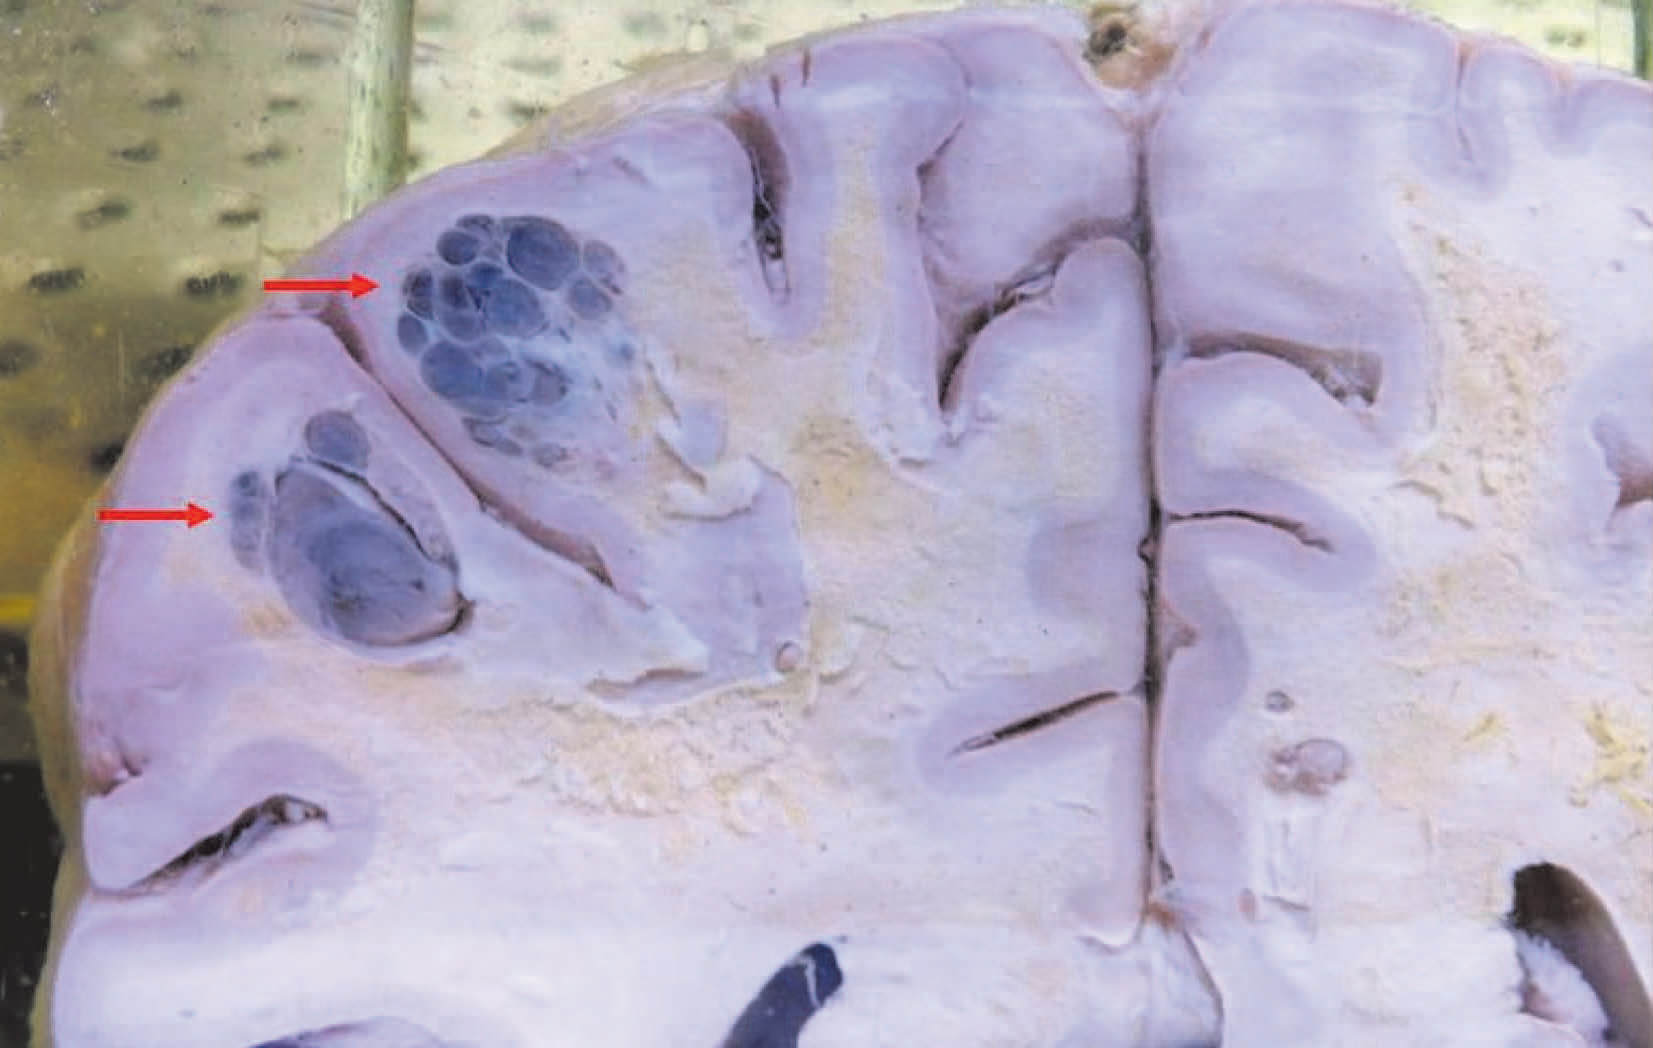
\includegraphics{./images/Image00146.jpg}
 \captionsetup{justification=centering}
 \caption{大脑皮层髓肉瘤(箭头所示)}
 \label{fig9-5}
  \end{figure} 

\paragraph{临床表现}
主要症状为发热、乏力、进行性贫血和出血倾向,脾和淋巴结肿大不如淋巴母细胞白血病。多见于成年人,随年龄增加,发病率升高,中位年龄为50岁。

\subsection{慢性白血病}

\subsubsection{慢性淋巴细胞性白血病和小淋巴细胞性淋巴瘤}

慢性淋巴细胞性白血病和小淋巴细胞性淋巴瘤(chronic lymphocytic
leukaemia/small lymphocytic
lymphoma,CLL/SLL)实际上是同一种肿瘤,其差别仅是累及外周血的程度不同。外周血中有大量瘤细胞(≥5$\times 10^9$
/L)时称慢性淋巴细胞性白血病,没有白血病表现的病例称小淋巴细胞性淋巴瘤。患者年龄通常大于50岁,男多于女。大多数患者诊断时表现为白血病。

\paragraph{病理变化}
淋巴结肿大,结构破坏,以假滤泡方式规则分布的淡染区域构成了增殖中心,其内有较大的细胞,周围是小淋巴细胞组成的深染背景。该结构对CLL/SLL具有诊断意义。病变以小淋巴细胞为主,较正常淋巴细胞稍大,染色质块状,核圆形,核分裂活性常很低。增殖中心由前淋巴细胞和副免疫母细胞构成,呈一系列小、中、大细胞。除淋巴结外,肿瘤常侵犯骨髓、脾和肝。在骨髓和外周血涂片中,CLL是小淋巴细胞,染色质块状,胞浆少。煤球(smudge)或篮球(basket)细胞是血涂片中见到的典型细胞。CLL/SLL是一种成熟的外周B细胞肿瘤,表达B细胞标记,如CD19、CD20、CD79a、PAX5、CD23,表达免疫球蛋白(IgM、IgD)轻链κ或λ。肿瘤细胞也表达T细胞相关抗原CD5。

\paragraph{临床表现}
90%的CLL/SLL病人在50岁以上发病。起病十分缓慢,往往无自觉症状。早期可能有乏力疲惫,后期出现食欲减退、消瘦、低热、盗汗及贫血等症状。淋巴结肿大常首先引起病人注意。50%~70%病人有轻至中度脾大。白细胞>10$\times 10^9$
/L,超过100$\times 10^9$
/L者不少。骨髓显示有核细胞增生活跃,淋巴细胞≥40%,以成熟淋巴细胞为主。约50%病人有染色体异常。12号染色体出现三倍体的情况可见于20%的病例。CLL/SLL的病程和预后差异很大,大部分患者在诊断后生存10年以上。中位生存时间是4~6年。

\subsubsection{慢性髓性白血病}

慢性髓性白血病又称慢性粒细胞性白血病,属于骨髓增殖性肿瘤,任何年龄均可发病,以中年最多见,男性略多于女性。大多数病人因急变而死亡。

\paragraph{细胞遗传学}
90%以上的慢性髓性白血病有特征性t(9;22)(q34;q11)易位,形成Ph1染色体。这种易位使22号染色体长臂上的BCR基因序列与9号染色体长臂上的ABL1基因序列融合,形成BCR/ABL1融合基因,该基因蛋白产物具有酪氨酸激酶活性,放大生长信号,促进细胞增殖。PCR检查BCR/ABL1融合基因灵敏度达1/106,对微小残留病灶的检测很有帮助。

\paragraph{病理变化}
白细胞数明显增高,常超过20$\times 10^9$/L,晚期可达100$\times 10^9$
/L以上。血涂片中性粒细胞显著增多,可见各阶段粒细胞,以中性中幼、晚幼和杆状核粒细胞居多;原始细胞一般为1%~3%,不超过10%。嗜酸、嗜碱粒细胞增多,后者有助于诊断。骨髓增生明显至极度活跃,以粒细胞为主,粒∶红比例可增至(10~50)∶1,其中中性中幼、晚幼级杆状核粒细胞明显增多。

\paragraph{临床表现}
病程发展缓慢,最初症状无特异性,主要为疲劳、衰弱、体重下降,可有贫血和明显的脾肿大。因无根治性治疗方法,大多数患者从慢性期或是突然进展为急变期或是经过一个过渡性的加速期后进入急变期,有些病例于加速期内死亡而无急变期。未经治疗的中位生存时间为2~3年。化疗后中位生存期约4年。5年生存率25%~50%。

\section*{复习与思考}

{一、名词解释}

R-S细胞 镜影细胞 绿色瘤 Ph1染色体 Auer小体

{二、问答题}

1. 试述霍奇金淋巴瘤的诊断要点。

2. 霍奇金淋巴瘤和非霍奇金淋巴瘤在临床和病理上有何异同?

3. 急、慢性粒细胞性白血病在临床和病理上有何差异?